\usetheme{opc}
\usepackage[]{appendixnumberbeamer}

% Font
\RequirePackage{mathpazo}
%\RequirePackage{fontspec}
%\setsansfont{Beteckna}
%\setsansfont{Noto Sans}
%\setsansfont{Futura LT}

%% Graphics
%\RequirePackage{shellesc}
\RequirePackage{tikz}
\usetikzlibrary{
%    arrows, 
%    arrows.meta,
%    backgrounds,
%    calc,
%    chains,
%    decorations,
%    decorations.markings,
%    external,
%    fit,
%    matrix,
    patterns,
%    positioning,
%    scopes,
%    shapes,
%    shapes.geometric,
%    fadings
}
%\tikzexternalize[prefix=tikzfigures/]
\input{tikzsettings}
%% Pgfplots
%\RequirePackage{pgfplots}
%\usepgfplotslibrary{patchplots, groupplots}
%\input{pgfplotssettings}
%% Circuits symbols
%\input{circuit_symbols}

% Code listings
\usepackage{listings}
\lstset{
    breaklines = true,
    %breakatwhitespace = true,
    language=[5.3]Lua,
    backgroundcolor = \color{blue!10!white},
    basicstyle = \small\ttfamily,
    keywordstyle = \color{blue},
    commentstyle = \color{red},
    stringstyle = \color{green!70!black},
    showstringspaces = false,
    tabsize = 4,
    gobble = 8,
    numbers = none,
    emph = {
        layout,
        parameters,
        config,
        pointarray,
        path,
        geometry,
        geometry.rectangle, 
        geometry.rectanglebltr, 
        geometry.polygon, 
        geometry.via, 
        geometry.viabltr, 
        geometry.contact, 
        geometry.contactbltr, 
        geometry.path, 
        pcell.setup, 
        pcell.add_cell_reference, 
        pcell.create_layout, 
        pcell.process_args, 
        pcell.check_args,
        pcell.add_parameter,
        pcell.add_parameters,
        pcell.get_parameters,
        object.create,
        object.translate,
        object.add_child,
        object.merge_into,
        get_anchor,
        move_anchor,
        translate,
        merge_into,
        flipx,
        flipy,
        add_child,
        add_child_reference,
        add_child_link,
        generics,
        generics.metal,
        generics.via,
        generics.contact,
        generics.other,
        generics.mapped,
        util.xmirror,
        util.make_insert_xy,
        posvals,
        even,
        odd,
        interval,
        set,
        inf
    },
    emphstyle = \color{blue!60!green}\bfseries,
    %belowskip=-0.2\baselineskip
}
\lstnewenvironment{luacode}{}{}
\newcommand{\luainline}[1]{\lstinline!#1!}
%\lstnewenvironment{shellcode}{\lstset{keywordstyle = \relax, commentstyle = \relax, stringstyle = \relax, identifierstyle = \relax, breakautoindent = false}}{}

% Units
\RequirePackage[per-mode=fraction, range-phrase=\ ---\ , exponent-product = \cdot]{siunitx}
\DeclareSIUnit{\dBc}{dBc}
\DeclareSIUnit{\dBchz}{dBc/Hz}

% Maths
\usepackage{amsmath}
\usepackage{IEEEtrantools}

% Tables
\usepackage{tabu, array, longtable, booktabs, makecell}

\usepackage{csquotes}


\title{OpenPCells}
\subtitle{Technical Documentation and Implementation Notes}
\author{Patrick Kurth}

\begin{document}
\maketitle
\section{Technology Mapping}
Mapping from generic cell descriptions to technology-specific data has to perform several steps:
\begin{itemize}
    \item resolve relative metal numbering
    \item split up via stacks
    \item translate via rectangles to via arrays
    \item map all remaining\footnote{The via translation already generates technology-specific layers.} layers
\end{itemize}

Figure \ref{fig:techtranslation} shows the technology translation from generic to specific layers. The process is discussed in detail further on in this document.
This example technology has 7 metal layers (labeled \enquote{M1} to \enquote{M7}), therefor \enquote{M-2} points to \enquote{M6}.
\begin{figure}[htb]
    \centering
    \begin{tikzpicture}
        [
            node distance = 2cm
        ]
        \node[state]                        (initial)  {Shape \nodepart{two} Polygon: \\\enquote{M-2} \nodepart{three} Via: \\\enquote{viaM-2M-4}};
        \node[state, right = of initial]    (metal)    {Shape \nodepart{two} Polygon: \\\enquote{M6}  \nodepart{three} Via: \\\enquote{viaM4M6}};
        \node[state, right = of metal]      (via)      {Shape \nodepart{two} Polygon: \\\enquote{M6} \nodepart{three} Via: \\\enquote{viaM4M5}\\\enquote{viaM5M6}};
        \node[state, right = of via]        (layer)    {Shape \nodepart{two} Polygon: \\\enquote{met6} \nodepart{three} Via: \\\enquote{V4}\\\enquote{V5}};
        % arrows
        \draw[tip]  (initial) -- node[above, align = center] {metal\\ translation} (metal);
        \draw[tip]  (metal)   -- node[above, align = center] {via\\ splitting}     (via);
        \draw[tip]  (via)     -- node[above, align = center] {layer\\ mapping} node[below, align = center] {via\\ arrayzation} (layer);
    \end{tikzpicture}
    \caption{Technology translation}
    \label{fig:techtranslation}
\end{figure}
Cell developers have to have a possibility of specifying generic layers (such as \enquote{gate}), since there can not be any technology-specific information in the
cells. This is achieved by using the generics module. The structures provided by this are crucial for the technology translation. Table \ref{tab:generics} shows the
currently available generics.

\begin{table}
    \centering
    \begin{tabular*}{\textwidth}{@{}l@{\extracolsep{\fill}}p{5cm}@{\extracolsep{\fill}}p{6cm}@{}}
        \toprule
        generics & Meaning & Action \\
        \midrule
        metal    & Any metal (including local interconnects) & Resolve relative numbering \\
        via      & A via between two metals & Remove dummy shape and place cuts \\
        contact  & A conctact from the first metal to a semiconductor layer & Remove dummy shape and place cuts \\
        other    & Anything that is nothing of the above & Perform regular layer mapping \\
        \midrule
        mapped   & Already mapped layer (real process layer) & Not to be used by cells, generated by technology translation \\
        \bottomrule
    \end{tabular*}
    \caption{Available generics}
    \label{tab:generics}
\end{table}

\subsection{Metal Numbering}
For some cells like inductors it is customary to specify things like \emph{last metal} or a metal relative to another. This has to be resolved for further
processing, which is done in this step. Currently, only negative numbers (such as \enquote{M-1}) are being processed into something like \enquote{M8} (depending on
the total number of metals in the technology).
\subsection{Via Splitting}
It is allowed the create via stacks, that is vias with non-adjacent metals. These have to split up into several shapes before via arrayzation.
\subsection{Via Arrayzation}
Via geometries can't be inside generic PCells, since these vary from technology to technology. For this reason, only rectangular areas where vias are to be placed in
a cell are specified. The technology translation then must create the actual via shapes, as shown in figure \ref{fig:viatranslation}.
\begin{wrapfigure}[11]{r}{5.8cm}
    \centering
    \begin{tikzpicture}[scale = 2]
        \def\viaxsize{0.2}
        \def\viaysize{0.2}
        \def\viaxspace{0.1}
        \def\viayspace{0.2}
        \def\vianumx{2}
        \def\vianumy{3}
        \def\viaxencl{0.1}
        \def\viayencl{0.1}
        \def\shiftx{1.8}
        \draw[thick, pattern = north west lines] 
            (
                {-0.5 * (\vianumx * \viaxsize + (\vianumx - 1) * \viaxspace + 2 * \viaxencl)},
                {-0.5 * (\vianumy * \viaysize + (\vianumy - 1) * \viayspace + 2 * \viayencl)}
            )
            rectangle 
            (
                { 0.5 * (\vianumx * \viaxsize + (\vianumx - 1) * \viaxspace + 2 * \viaxencl)},
                { 0.5 * (\vianumy * \viaysize + (\vianumy - 1) * \viayspace + 2 * \viayencl)}
            );
        \draw[densely dotted] 
            (
                {\shiftx + -0.5 * (\vianumx * \viaxsize + (\vianumx - 1) * \viaxspace + 2 * \viaxencl)},
                {-0.5 * (\vianumy * \viaysize + (\vianumy - 1) * \viayspace + 2 * \viayencl)}
            )
            rectangle 
            (
                {\shiftx +  0.5 * (\vianumx * \viaxsize + (\vianumx - 1) * \viaxspace + 2 * \viaxencl)},
                { 0.5 * (\vianumy * \viaysize + (\vianumy - 1) * \viayspace + 2 * \viayencl)}
            );
        \foreach \x in {1, ..., \vianumx}
        {
            \foreach \y in {1, ..., \vianumy}
            {
                \draw[thick, pattern = crosshatch dots] 
                    (
                        {\shiftx + (\x - 0.5 * (\vianumx - 1) - 1) * (\viaxsize + \viaxspace) - 0.5 * \viaxsize}, 
                        {(\y - 0.5 * (\vianumy - 1) - 1) * (\viaysize + \viayspace) - 0.5 * \viaysize}
                    ) rectangle 
                    (
                        {\shiftx + (\x - 0.5 * (\vianumx - 1) - 1) * (\viaxsize + \viaxspace) + 0.5 * \viaxsize}, 
                        {(\y - 0.5 * (\vianumy - 1) - 1) * (\viaysize + \viayspace) + 0.5 * \viaysize}
                    );
            }
        }
        \draw[tip] 
            ({ 0.05 + 0.5 * (\vianumx * \viaxsize + (\vianumx - 1) * \viaxspace + 2 * \viaxencl)}, 0)
                -- node[above, align = center] { Generate \\ Via Array } 
            ({-0.05 + \shiftx - 0.5 * (\vianumx * \viaxsize + (\vianumx - 1) * \viaxspace + 2 * \viaxencl)}, 0);
        % legend
        \draw[thick, pattern = north west lines] 
            (
                {-0.5 * (\vianumx * \viaxsize + (\vianumx - 1) * \viaxspace + 2 * \viaxencl)},
                {-0.5 * (\vianumy * \viaysize + (\vianumy - 1) * \viayspace + 2 * \viayencl) - 0.2}
            )
            rectangle 
            (
                {-0.5 * (\vianumx * \viaxsize + (\vianumx - 1) * \viaxspace + 2 * \viaxencl) + 0.2},
                {-0.5 * (\vianumy * \viaysize + (\vianumy - 1) * \viayspace + 2 * \viayencl) - 0.4}
            );
        \node[anchor = west]
            at
            (
                {-0.5 * (\vianumx * \viaxsize + (\vianumx - 1) * \viaxspace + 2 * \viaxencl) + 0.3},
                {-0.5 * (\vianumy * \viaysize + (\vianumy - 1) * \viayspace + 2 * \viayencl) - 0.3}
            )
            {Generic Layer};
        \draw[thick, pattern = crosshatch dots] 
            (
                {-0.5 * (\vianumx * \viaxsize + (\vianumx - 1) * \viaxspace + 2 * \viaxencl)},
                {-0.5 * (\vianumy * \viaysize + (\vianumy - 1) * \viayspace + 2 * \viayencl) - 0.6}
            )
            rectangle 
            (
                {-0.5 * (\vianumx * \viaxsize + (\vianumx - 1) * \viaxspace + 2 * \viaxencl) + 0.2},
                {-0.5 * (\vianumy * \viaysize + (\vianumy - 1) * \viayspace + 2 * \viayencl) - 0.8}
            );
        \node[anchor = west]
            at
            (
                {-0.5 * (\vianumx * \viaxsize + (\vianumx - 1) * \viaxspace + 2 * \viaxencl) + 0.3},
                {-0.5 * (\vianumy * \viaysize + (\vianumy - 1) * \viayspace + 2 * \viayencl) - 0.7}
            )
            {Specific Layer};
    \end{tikzpicture}
    \caption{Example of via arrayzation}
    \label{fig:viatranslation}
\end{wrapfigure}
For this process, the technology file has to define the size of the individual cuts (width and height), the spacing in x- and y-direction as well as the minimum
enclosure of the surrounding layers (metals). The generated cuts fullfill the following equations:
\begin{IEEEeqnarray*}{rCl}
    \text{width} &=& N_x \cdot W + (N_x - 1) \cdot S_x + 2 \cdot E_x \\
    \text{height} &=& N_y \cdot H + (N_y - 1) \cdot S_y + 2 \cdot E_y 
\end{IEEEeqnarray*}
For the generation of the cuts, these equations are solved for $N_x$ and $N_y$.
\subsection{Layer Mapping}
The stage of layer mapping is the last of the technology translation, as some earlier stages also create to-be-mapped layers (for instance contacts will always
generate instances of \enquote{M1}). Layer mapping is a simple process, as no shapes have to be modified. Here only \enquote{mapped} and \enquote{other} layers
remain, where the former are naturally ignored.

\section{Cell Parameterization}
Cell parameters are defined in the \luainline{parameters()} function via the \luainline{pcell} module. It uses one state to store all parameters, so everytime a
layout is created, the parameters have to be defined first. A different approach to this would be to store all loaded parameters and retrieve the right ones when a
cell layout is created. Since currently there are no performance issues, no storing is made as code complexity increases (one has to check if loaded parameters exist
etc.). 

\section{Shape Reduction}
The generation process generates a lot of shapes that overlap partially or fully. Certain combinations of shapes can be merged, reducing the overall complexity
(while maintaining the functionality of the layout, of course). Currently, a simple algorithm to merge rectangles is implemented, as rectanges usually make up
the main part of a layout for integrated circuits. Union of polygons is much more complex, logic- and computation-wise.

The implemented algorithm simply checks if two rectangles can be merged into a rectangle by looking for certain topologies. All possible cases are shown in
figure~\ref{fig:merge_rectangle_toplogies}. Two independent checks are run for x and y, only x topologies are shown.
\begin{figure}
    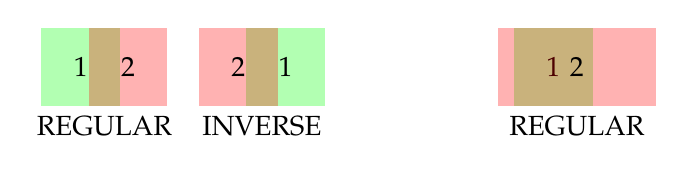
\begin{tikzpicture}
        [
            single/.style = {draw=none, text opacity = 1, fill opacity=0.3, rectangle, inner sep = 0pt, minimum width = 1cm, minimum height = 1cm},
            double/.style = {draw=none, text opacity = 1, fill opacity=0.3, rectangle, inner sep = 0pt, minimum width = 2cm, minimum height = 1cm}
        ]
        \def\xpos{0}
        \node[single, fill = green] at ({\xpos - 0.3}, 0) {1};
        \node[single, fill = red] at ({\xpos + 0.3}, 0) {2};
        \node[below] at (\xpos, -0.5) {REGULAR};
        \def\xpos{2}
        \node[single, fill = green] at ({\xpos + 0.3}, 0) {1};
        \node[single, fill = red] at ({\xpos + -0.3}, 0) {2};
        \node[below] at (\xpos, -0.5) {INVERSE};
        \def\xpos{6}
        \node[single, fill = green] at ({\xpos - 0.3}, 0) {1};
        \node[double, fill = red] at ({\xpos - 0.0}, 0) {2};
        \node[below] at (\xpos, -0.5) {REGULAR};
    \end{tikzpicture}
    \caption{Possible topologies for rectangle union}
    \label{fig:merge_rectangle_toplogies}
\end{figure}
\end{document}

% vim: ft=tex
